  \documentclass{beamer}

  \usepackage[utf8]{inputenc}


  %Information to be included in the title page:
  \title{Projeto de Arquitetura de Software}
  \author{Weblioteca}
  \institute{Universidade Estadual de Maringá}
  \date{2020}


  %--------------------------------------------------
  %--------------------------------------------------
  %--------------------------------------------------
  \begin{document}
  %--------------------------------------------------
  %--------------------------------------------------
  %--------------------------------------------------
  \frame{\titlepage}

  \begin{frame}
  \frametitle{Tecnologias empregadas}

\begin{tabular}{c|c}
     & Linguagem: C\# \\ 
     & .NET Framework\\ 
     & IDE Visual Studio\\ 
\end{tabular}

  \end{frame}
  %--------------------------------------------------
  %--------------------------------------------------
  %--------------------------------------------------

  \begin{frame}

  \frametitle{Estilos arquiteturais}

  

  \end{frame}
  %--------------------------------------------------
  %--------------------------------------------------
  %--------------------------------------------------
  \begin{frame}

  \frametitle{Padrão de Projeto}

  Quando necessita-se de variantes de um algoritmo;

  \end{frame}
%--------------------------------------------------
%--------------------------------------------------
%--------------------------------------------------
\begin{frame}
\frametitle{Diagrama de Componentes}

\begin{figure}[!ht]
\centering
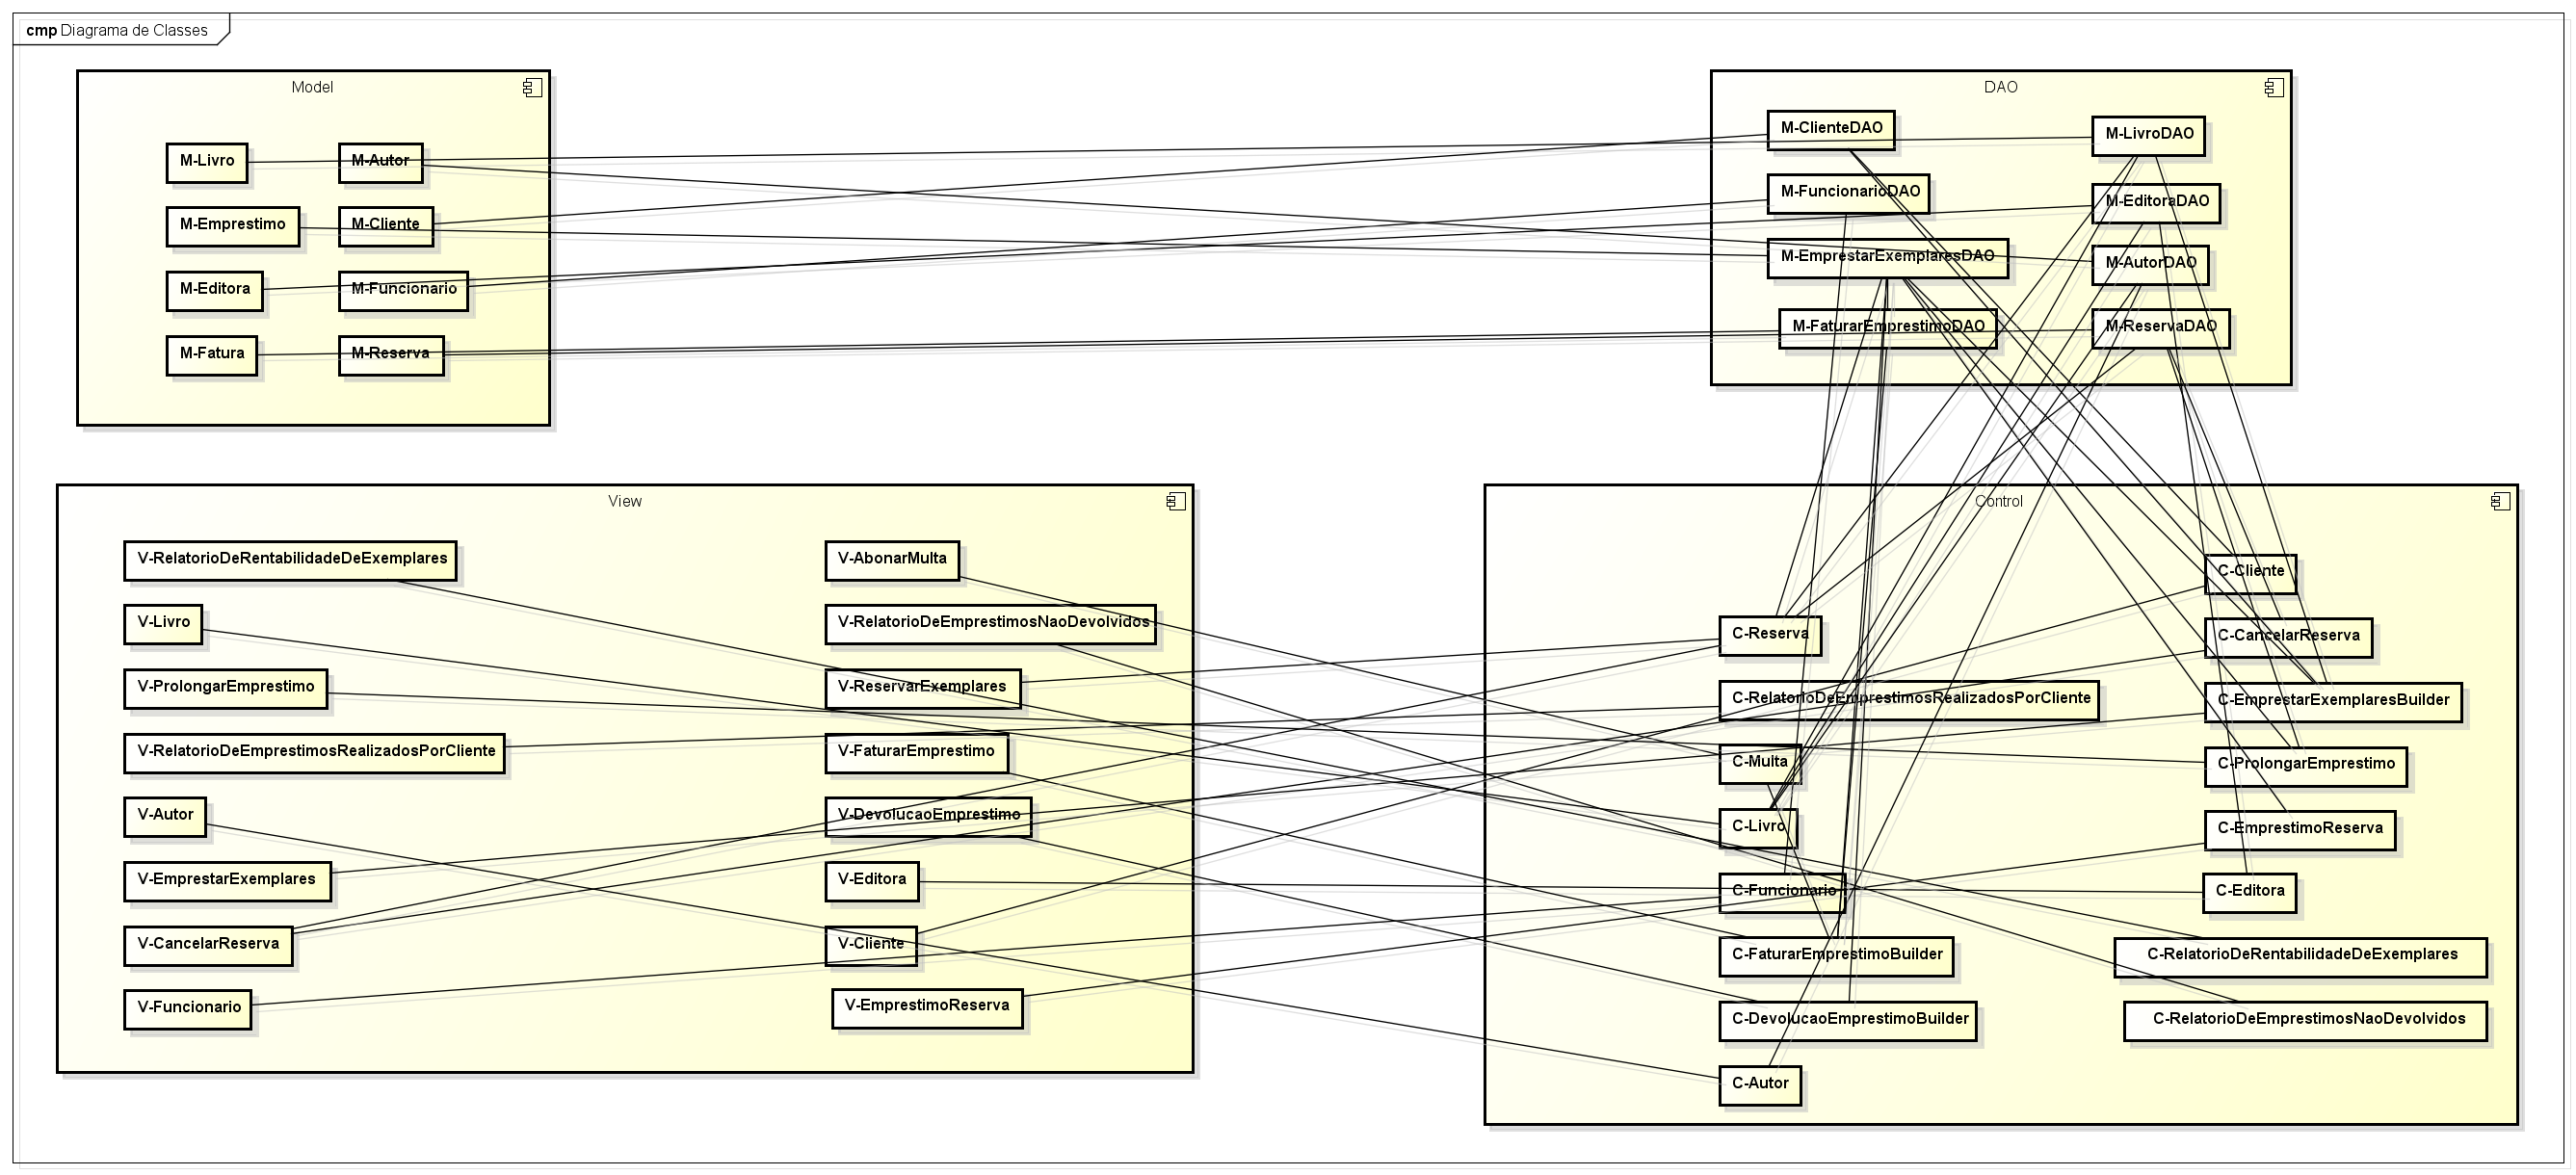
\includegraphics[width=10cm]{Diagrama_de_Componentes.png}
\end{figure}

\end{frame}
%--------------------------------------------------
%--------------------------------------------------
%--------------------------------------------------
\begin{frame}

\frametitle{Diagrama de Classes de Projeto}
\begin{figure}[!ht]
\centering
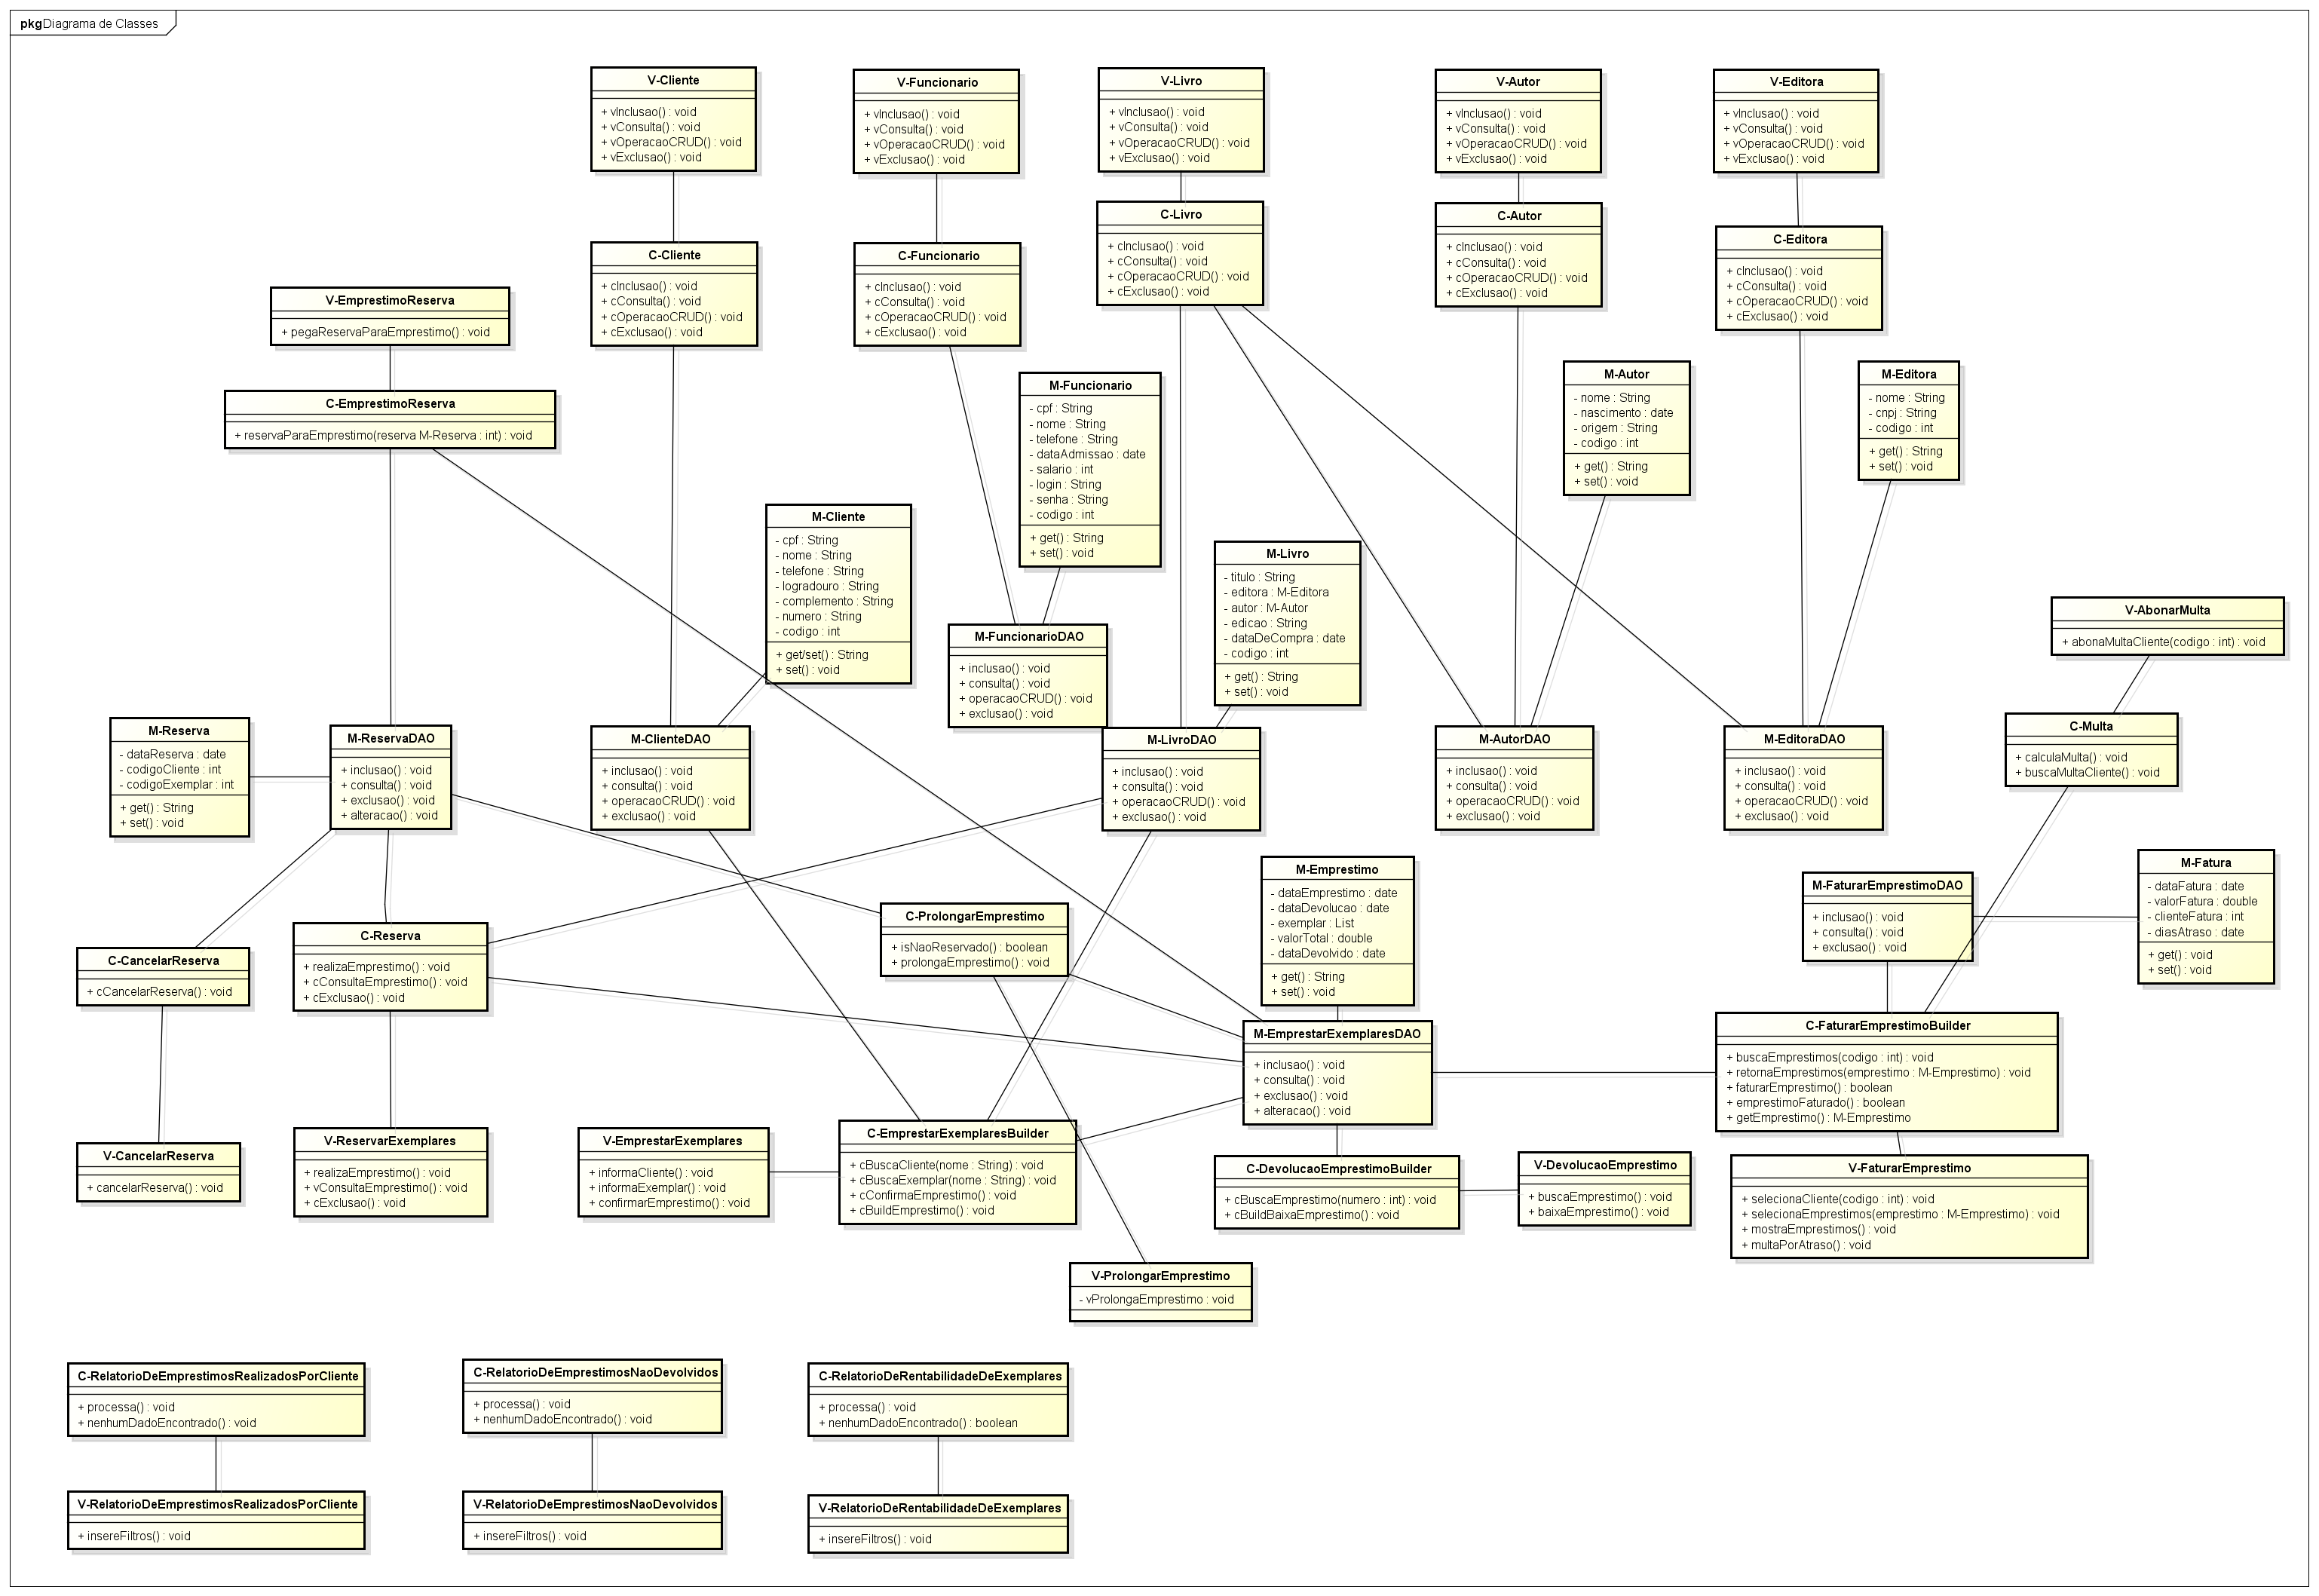
\includegraphics[width=10cm]{Diagrama_de_Classes.png}
\end{figure}

\end{frame}
  %--------------------------------------------------
  %--------------------------------------------------
  %--------------------------------------------------
\begin{frame}

\frametitle{Diagrama de Sequência}
\begin{figure}[!ht]
\centering
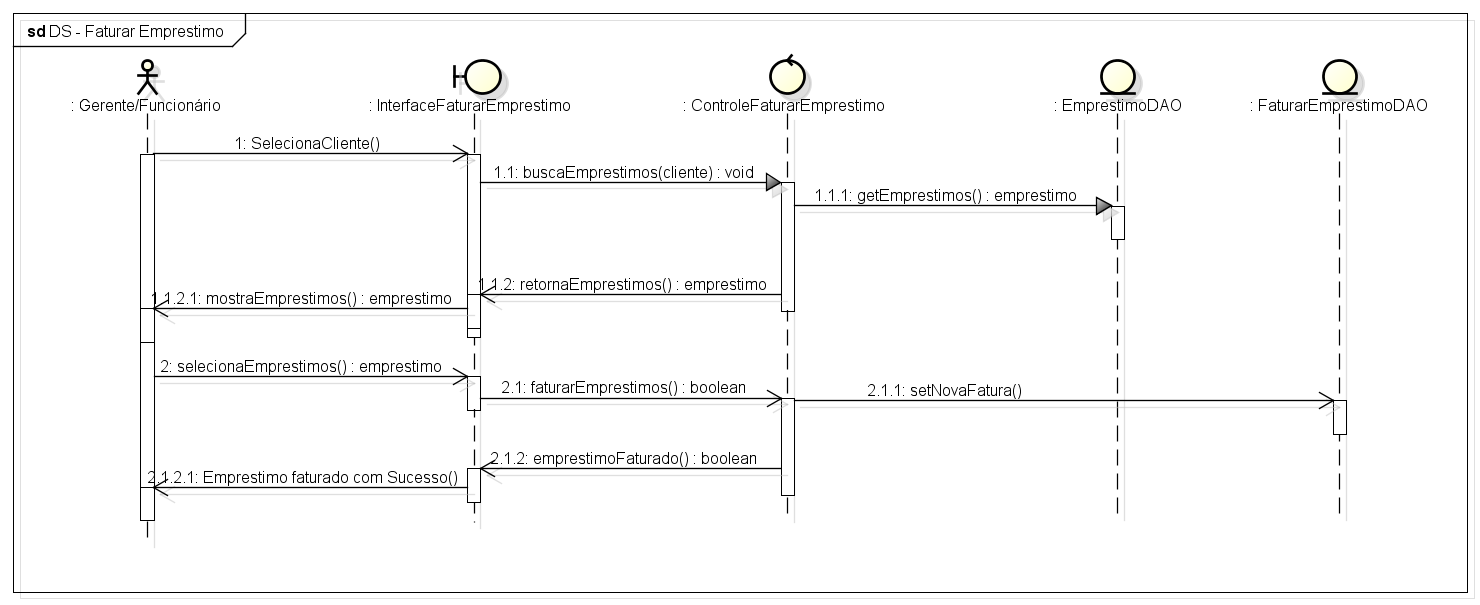
\includegraphics[width=10cm]{ds-fatura-emprestimo-henrique.png}

\end{figure}

\end{frame}
  %--------------------------------------------------
  %--------------------------------------------------
  %--------------------------------------------------
\begin{frame}

\frametitle{Diagrama de Atividade}
\begin{figure}[!ht]
\centering
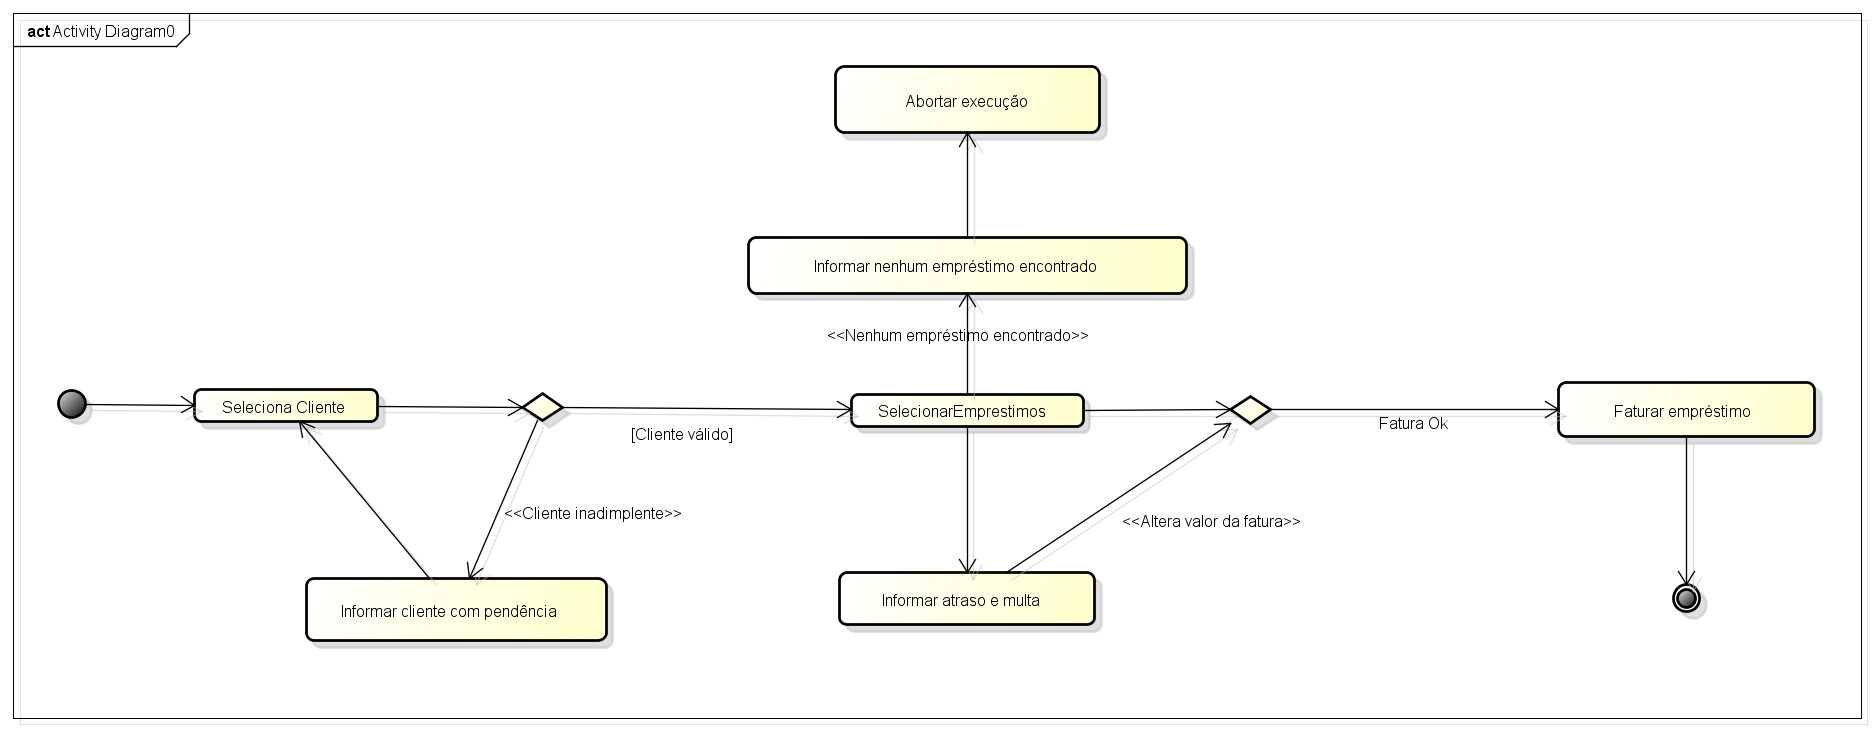
\includegraphics[width=10cm]{da-fatura-emprestimo-henrique.png}

\end{figure}

\end{frame}

  %--------------------------------------------------
  %--------------------------------------------------
  %--------------------------------------------------
\begin{frame}

\frametitle{Weblioteca}
\begin{figure}[!ht]
\centering
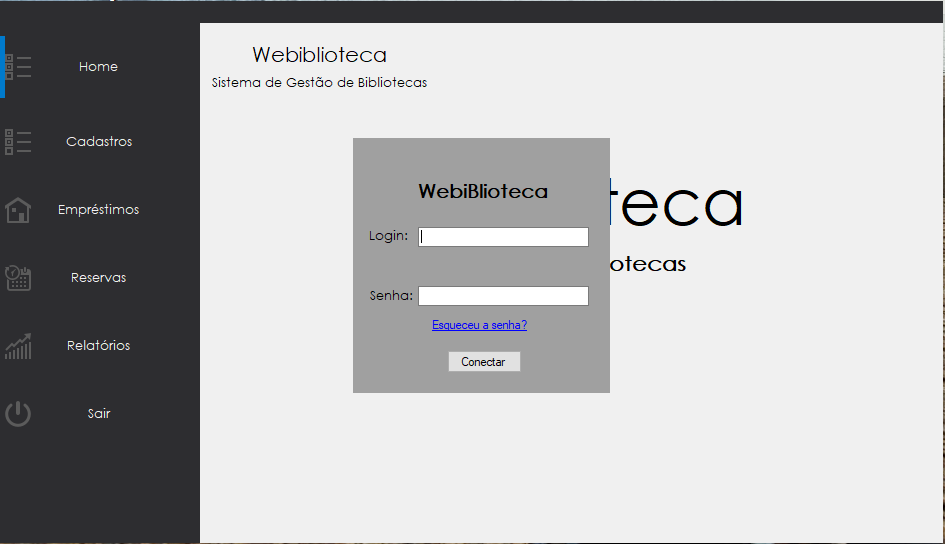
\includegraphics[width=10cm]{codigo/home.png}

\end{figure}

\end{frame}
  %--------------------------------------------------
  %--------------------------------------------------
  %--------------------------------------------------
\begin{frame}
\frametitle{RF003 - Manter Livros}
\begin{figure}[!ht]
\centering
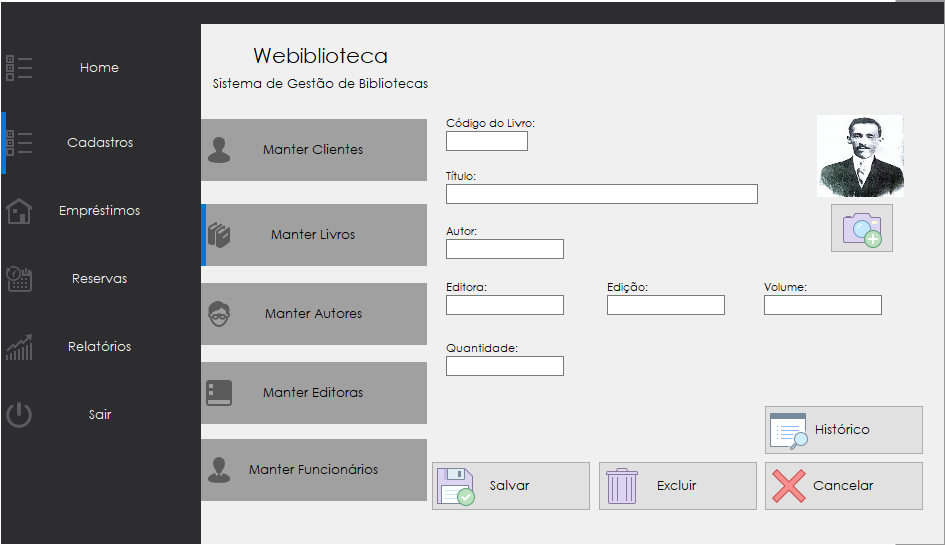
\includegraphics[width=10cm]{codigo/img1.png}
\end{figure}

\end{frame}
  %--------------------------------------------------
  %--------------------------------------------------
  %--------------------------------------------------
\begin{frame}

\frametitle{RF008 - Faturar Empréstimo}
\begin{figure}[!ht]
\centering
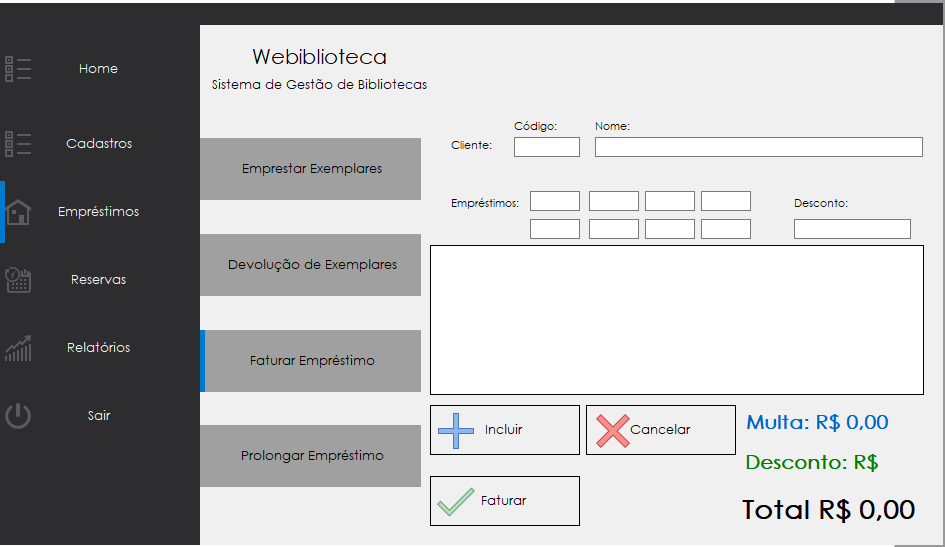
\includegraphics[width=10cm]{codigo/img2.png}
\end{figure}

\end{frame}
  %--------------------------------------------------
  %--------------------------------------------------
  %--------------------------------------------------
\begin{frame}

\frametitle{RF011 - Prolongar Empréstimo}
\begin{figure}[!ht]
\centering
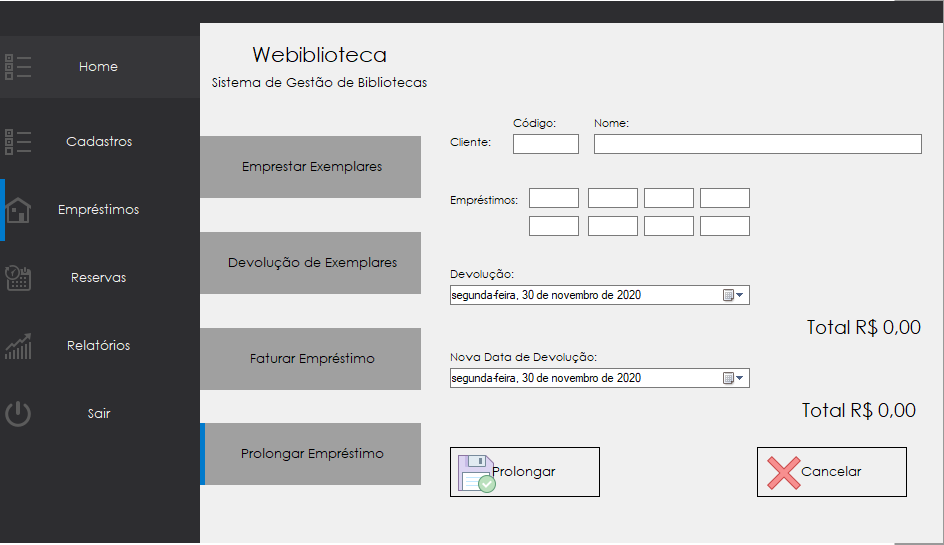
\includegraphics[width=10cm]{codigo/img3.png}
\end{figure}

\end{frame}
  %--------------------------------------------------
  %--------------------------------------------------
  %--------------------------------------------------
\begin{frame}

\frametitle{RF012 - Abonar Multa}
\begin{figure}[!ht]
\centering
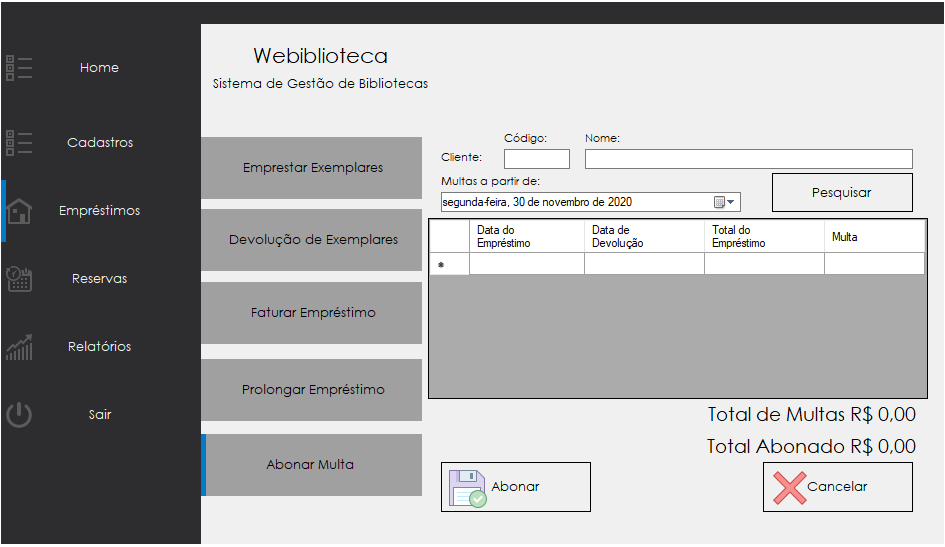
\includegraphics[width=10cm]{codigo/img4.png}
\end{figure}

\end{frame}
  %--------------------------------------------------
  %--------------------------------------------------
  %--------------------------------------------------
\begin{frame}

\frametitle{RF015 - Relatório de Rentabilidade de Exemplares}
\begin{figure}[!ht]
\centering
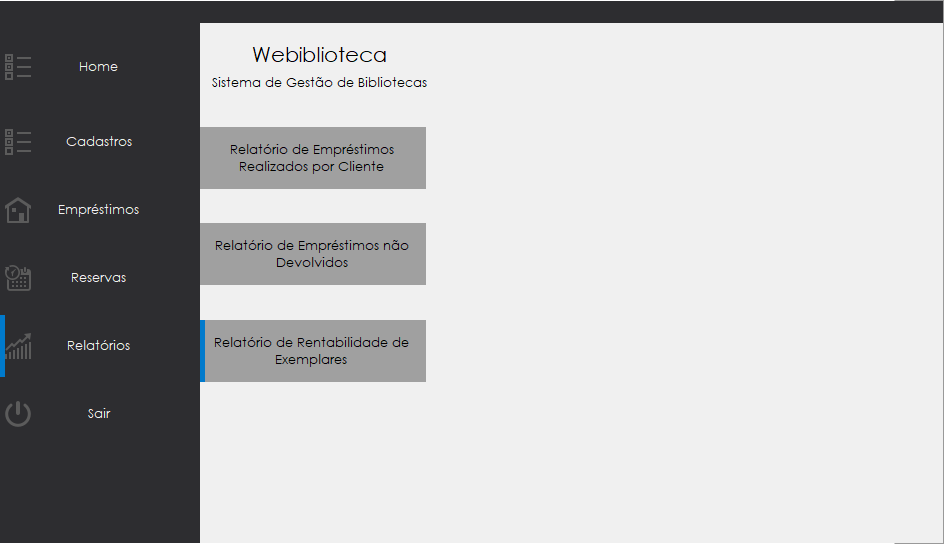
\includegraphics[width=10cm]{codigo/img5.png}
\end{figure}

\end{frame}
  %--------------------------------------------------
  %--------------------------------------------------
  %--------------------------------------------------
\begin{frame}

\frametitle{RF016 - Empréstimo Reserva}
\begin{figure}[!ht]
\centering
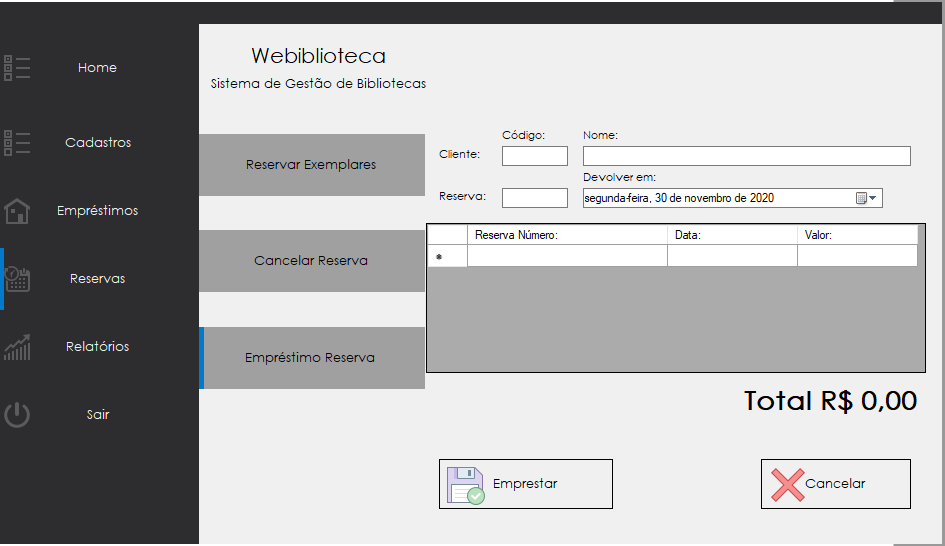
\includegraphics[width=10cm]{codigo/img6.png}
\end{figure}

\end{frame}
  %--------------------------------------------------
  %--------------------------------------------------
  %--------------------------------------------------
  \begin{frame}

  \frametitle{Diagrama de Implantação}

  \centering
  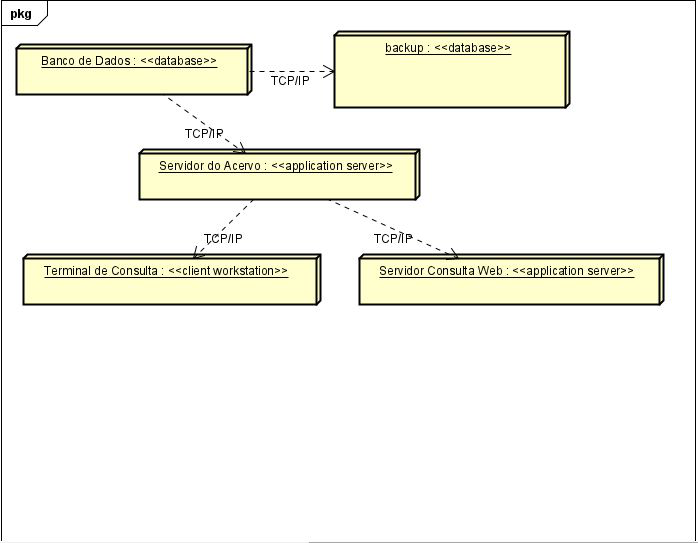
\includegraphics[width = 10cm]{Diagramas_de_Implantacao.png}
   
  \end{frame} 
 
%--------------------------------------------------
%--------------------------------------------------
%--------------------------------------------------
\begin{frame}

\frametitle{Fim}

Perguntas?

\end{frame}
%--------------------------------------------------
%--------------------------------------------------
%--------------------------------------------------
\end{document}